\section{Constructions}\label{sec:constructions}

We write the line $\ell_m$ as $a_mx+b_my=c_m$ with integer coefficients. Each polygon is given by the
cyclic sequence of its vertices, where the vertex ``$p/q$'' is $\ell_p\cap\ell_q$. Consecutive vertices
share a line, which carries the side between them. All data, including vertex coordinates as exact
rationals, are in \texttt{data/polyN.json} and \texttt{lean/Main.lean}.

\begin{table}[h]
\centering\small
\begin{tabular}{@{}r>{\raggedright\arraybackslash}p{0.83\textwidth}@{}}
\toprule
$n$ & lines $(a_m,b_m,c_m)$, $m=1,\dots,n$\\
\midrule
$7$ & $(-6,17,-74)$, $(0,-19,-95)$, $(-19,14,-98)$, $(4,-7,8)$, $(-19,13,-44)$, $(8,11,41)$, $(-6,2,-41)$\\
$9$ & $(-22,6,-118)$, $(-14,-23,103)$, $(18,-2,91)$, $(11,-6,-43)$, $(-24,1,-136)$, $(27,23,49)$,
      $(-3,8,-149)$, $(14,-2,-14)$, $(16,21,-33)$\\
$11$ & $(-39,31,-51)$, $(1,50,7)$, $(-22,45,-264)$, $(12,-49,-212)$, $(-10,-49,-25)$, $(-16,48,31)$,
       $(48,-14,68)$, $(-19,46,-80)$, $(-50,3,89)$, $(17,47,93)$, $(15,48,37)$\\
$13$ & $(5,-19,255)$, $(17,11,229)$, $(-4,20,-1118)$, $(14,-14,106)$, $(19,4,126)$, $(3,-20,-505)$,
       $(-6,19,-402)$, $(10,17,78)$, $(20,-3,-68)$, $(-1,20,240)$, $(18,-8,29)$, $(7,-19,-397)$,
       $(-20,-3,-59)$\\
\bottomrule
\end{tabular}
\caption{The certified arrangements.}\label{tab:lines}
\end{table}

\paragraph{$n=7$, an $18$-gon.} The vertex cycle is
\begin{center}\small
1/2, 1/6, 6/7, 1/7, 1/3, 3/5, 1/5, 1/4, 4/5, 5/6, 2/6, 2/5, 5/7, 2/7, 2/3, 3/7, 4/7, 2/4.
\end{center}
It uses every intersection point except the three points of the triangle of lines $\{3,4,6\}$. Lines
$3,4,6$ each carry $2$ sides and the other lines carry $3$. The line pairs used form $K_7$ minus a
triangle, which is the extremal case of Proposition~\ref{prop:forced}(2).

\paragraph{$n=9$, a $33$-gon.} This uses all intersection points except those of the triangle of lines
$\{1,2,9\}$; the cycle is listed in \cref{app:cycles}.

\paragraph{$n=11$ and $n=13$.} Here the polygon is the alternating $2$-factor $G$ itself, which is a
single cycle of length $55$, respectively $78$; it is listed in \cref{app:cycles}. Each line carries
$(n-1)/2$ sides.

\begin{figure}[h]
\centering
\begin{minipage}{0.48\textwidth}\centering\resizebox{\textwidth}{!}{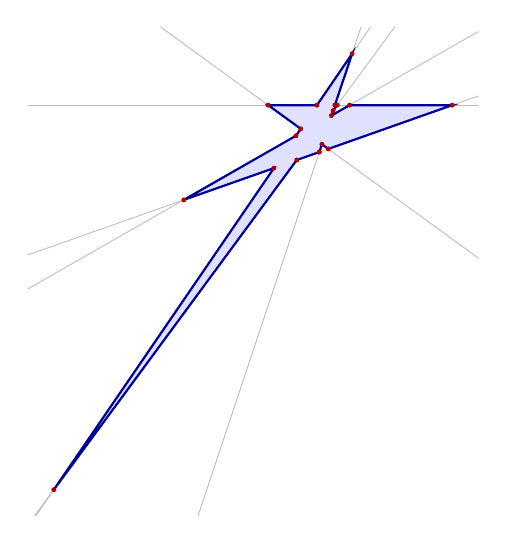
\begin{tikzpicture}
\clip (0,0) rectangle (5.725,6.200);
\draw[gray!55,line width=0.3pt] (-57.246,-16.892)--(62.970,25.538);
\draw[gray!55,line width=0.3pt] (-57.246,5.216)--(62.970,5.216);
\draw[gray!55,line width=0.3pt] (-45.597,-62.000)--(50.340,68.200);
\draw[gray!55,line width=0.3pt] (-57.246,-29.832)--(62.970,38.863);
\draw[gray!55,line width=0.3pt] (-42.316,-62.000)--(46.768,68.200);
\draw[gray!55,line width=0.3pt] (-57.246,49.070)--(62.970,-38.360);
\draw[gray!55,line width=0.3pt] (-18.503,-62.000)--(24.897,68.200);
\filldraw[fill=blue!12,draw=blue!60!black,line width=0.8pt] (5.392,5.216) -- (3.818,4.660) -- (3.737,4.719) -- (3.704,4.620) -- (3.417,4.519) -- (0.332,0.332) -- (3.127,4.416) -- (1.983,4.013) -- (3.407,4.827) -- (3.468,4.915) -- (3.054,5.216) -- (3.674,5.216) -- (4.120,5.868) -- (3.902,5.216) -- (3.931,5.216) -- (3.879,5.146) -- (3.859,5.085) -- (4.089,5.216) -- cycle;
\fill[red!70!black] (5.392,5.216) circle (0.9pt);
\fill[red!70!black] (3.818,4.660) circle (0.9pt);
\fill[red!70!black] (3.737,4.719) circle (0.9pt);
\fill[red!70!black] (3.704,4.620) circle (0.9pt);
\fill[red!70!black] (3.417,4.519) circle (0.9pt);
\fill[red!70!black] (0.332,0.332) circle (0.9pt);
\fill[red!70!black] (3.127,4.416) circle (0.9pt);
\fill[red!70!black] (1.983,4.013) circle (0.9pt);
\fill[red!70!black] (3.407,4.827) circle (0.9pt);
\fill[red!70!black] (3.468,4.915) circle (0.9pt);
\fill[red!70!black] (3.054,5.216) circle (0.9pt);
\fill[red!70!black] (3.674,5.216) circle (0.9pt);
\fill[red!70!black] (4.120,5.868) circle (0.9pt);
\fill[red!70!black] (3.902,5.216) circle (0.9pt);
\fill[red!70!black] (3.931,5.216) circle (0.9pt);
\fill[red!70!black] (3.879,5.146) circle (0.9pt);
\fill[red!70!black] (3.859,5.085) circle (0.9pt);
\fill[red!70!black] (4.089,5.216) circle (0.9pt);
\end{tikzpicture}}\\[2pt]
\small $18$ sides on $7$ lines\end{minipage}\hfill
\begin{minipage}{0.48\textwidth}\centering\resizebox{\textwidth}{!}{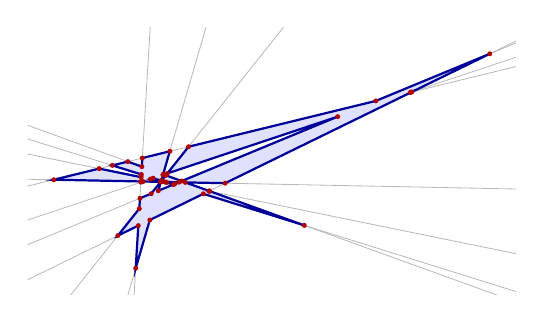
\begin{tikzpicture}
\clip (0,0) rectangle (6.200,3.387);
\draw[gray!55,line width=0.3pt] (-26.368,-33.868)--(30.165,37.255);
\draw[gray!55,line width=0.3pt] (-62.000,2.702)--(68.200,0.098);
\draw[gray!55,line width=0.3pt] (-62.000,-30.125)--(68.200,33.528);
\draw[gray!55,line width=0.3pt] (-62.000,-13.809)--(68.200,18.077);
\draw[gray!55,line width=0.3pt] (-62.000,14.435)--(68.200,-12.136);
\draw[gray!55,line width=0.3pt] (-62.000,-19.722)--(68.200,23.678);
\draw[gray!55,line width=0.3pt] (-8.603,-33.868)--(12.142,37.255);
\draw[gray!55,line width=0.3pt] (-62.000,-24.978)--(68.200,28.801);
\draw[gray!55,line width=0.3pt] (-0.680,-33.868)--(3.588,37.255);
\draw[gray!55,line width=0.3pt] (-62.000,24.572)--(68.200,-22.521);
\draw[gray!55,line width=0.3pt] (-62.000,21.349)--(68.200,-19.339);
\filldraw[fill=blue!12,draw=blue!60!black,line width=0.8pt] (1.688,1.429) -- (1.569,1.279) -- (1.426,1.220) -- (1.418,1.089) -- (1.145,0.746) -- (1.405,0.873) -- (1.372,0.332) -- (1.551,0.944) -- (2.231,1.277) -- (3.513,0.876) -- (2.312,1.310) -- (2.303,1.312) -- (2.305,1.313) -- (2.002,1.422) -- (2.508,1.412) -- (4.871,2.567) -- (4.859,2.564) -- (4.878,2.571) -- (5.868,3.055) -- (4.422,2.457) -- (2.043,1.875) -- (1.773,1.536) -- (3.937,2.257) -- (1.956,1.439) -- (1.754,1.512) -- (1.699,1.443) -- (1.748,1.427) -- (1.920,1.424) -- (1.865,1.401) -- (1.767,1.421) -- (1.851,1.395) -- (1.659,1.316) -- (1.692,1.429) -- (1.737,1.428) -- (1.694,1.436) -- (1.695,1.437) -- (1.694,1.436) -- (1.558,1.464) -- (1.593,1.476) -- (1.697,1.444) -- (1.718,1.517) -- (1.729,1.521) -- (1.720,1.524) -- (1.805,1.817) -- (1.456,1.731) -- (1.450,1.622) -- (1.273,1.686) -- (1.075,1.638) -- (1.444,1.523) -- (1.442,1.488) -- (0.908,1.597) -- (0.332,1.456) -- (1.438,1.434) -- (1.438,1.424) -- (1.465,1.433) -- cycle;
\fill[red!70!black] (1.688,1.429) circle (0.9pt);
\fill[red!70!black] (1.569,1.279) circle (0.9pt);
\fill[red!70!black] (1.426,1.220) circle (0.9pt);
\fill[red!70!black] (1.418,1.089) circle (0.9pt);
\fill[red!70!black] (1.145,0.746) circle (0.9pt);
\fill[red!70!black] (1.405,0.873) circle (0.9pt);
\fill[red!70!black] (1.372,0.332) circle (0.9pt);
\fill[red!70!black] (1.551,0.944) circle (0.9pt);
\fill[red!70!black] (2.231,1.277) circle (0.9pt);
\fill[red!70!black] (3.513,0.876) circle (0.9pt);
\fill[red!70!black] (2.312,1.310) circle (0.9pt);
\fill[red!70!black] (2.303,1.312) circle (0.9pt);
\fill[red!70!black] (2.305,1.313) circle (0.9pt);
\fill[red!70!black] (2.002,1.422) circle (0.9pt);
\fill[red!70!black] (2.508,1.412) circle (0.9pt);
\fill[red!70!black] (4.871,2.567) circle (0.9pt);
\fill[red!70!black] (4.859,2.564) circle (0.9pt);
\fill[red!70!black] (4.878,2.571) circle (0.9pt);
\fill[red!70!black] (5.868,3.055) circle (0.9pt);
\fill[red!70!black] (4.422,2.457) circle (0.9pt);
\fill[red!70!black] (2.043,1.875) circle (0.9pt);
\fill[red!70!black] (1.773,1.536) circle (0.9pt);
\fill[red!70!black] (3.937,2.257) circle (0.9pt);
\fill[red!70!black] (1.956,1.439) circle (0.9pt);
\fill[red!70!black] (1.754,1.512) circle (0.9pt);
\fill[red!70!black] (1.699,1.443) circle (0.9pt);
\fill[red!70!black] (1.748,1.427) circle (0.9pt);
\fill[red!70!black] (1.920,1.424) circle (0.9pt);
\fill[red!70!black] (1.865,1.401) circle (0.9pt);
\fill[red!70!black] (1.767,1.421) circle (0.9pt);
\fill[red!70!black] (1.851,1.395) circle (0.9pt);
\fill[red!70!black] (1.659,1.316) circle (0.9pt);
\fill[red!70!black] (1.692,1.429) circle (0.9pt);
\fill[red!70!black] (1.737,1.428) circle (0.9pt);
\fill[red!70!black] (1.694,1.436) circle (0.9pt);
\fill[red!70!black] (1.695,1.437) circle (0.9pt);
\fill[red!70!black] (1.694,1.436) circle (0.9pt);
\fill[red!70!black] (1.558,1.464) circle (0.9pt);
\fill[red!70!black] (1.593,1.476) circle (0.9pt);
\fill[red!70!black] (1.697,1.444) circle (0.9pt);
\fill[red!70!black] (1.718,1.517) circle (0.9pt);
\fill[red!70!black] (1.729,1.521) circle (0.9pt);
\fill[red!70!black] (1.720,1.524) circle (0.9pt);
\fill[red!70!black] (1.805,1.817) circle (0.9pt);
\fill[red!70!black] (1.456,1.731) circle (0.9pt);
\fill[red!70!black] (1.450,1.622) circle (0.9pt);
\fill[red!70!black] (1.273,1.686) circle (0.9pt);
\fill[red!70!black] (1.075,1.638) circle (0.9pt);
\fill[red!70!black] (1.444,1.523) circle (0.9pt);
\fill[red!70!black] (1.442,1.488) circle (0.9pt);
\fill[red!70!black] (0.908,1.597) circle (0.9pt);
\fill[red!70!black] (0.332,1.456) circle (0.9pt);
\fill[red!70!black] (1.438,1.434) circle (0.9pt);
\fill[red!70!black] (1.438,1.424) circle (0.9pt);
\fill[red!70!black] (1.465,1.433) circle (0.9pt);
\end{tikzpicture}}\\[2pt]
\small $55$ sides on $11$ lines\end{minipage}
\caption{Two of the certified polygons, drawn to scale. The grey lines are the arrangement, clipped
to a box around the polygon. Several sides are very short, so some corners are not resolved at this
scale; exact coordinates are in the data files.}\label{fig:polys}
\end{figure}

\paragraph{How they were found.} For $n=11,13$ we ran a simulated-annealing search over random real
arrangements, minimising the number of components of $G$. Theorem~\ref{thm:parity} predicts an odd number for
these $n$, and the search eventually reaches one component. The resulting coefficients were rounded
to small integers and re-checked with exact rational arithmetic.

For $n=7,9$ we sampled random integer arrangements and, for each triangle $\{a,b,c\}$ of lines, formed
the graph that pairs consecutive remaining intersection points on every line, leaving out
$\ell_a\cap\ell_b$, $\ell_b\cap\ell_c$ and $\ell_a\cap\ell_c$. We kept the arrangement when this graph
was a single cycle bounding a simple polygon.

The search method plays no role in correctness. Every polygon is verified directly, as described in
\cref{sec:formal}.

\begin{proof}[Proof of Theorem~\ref{thm:constructions}]
The four polygons are simple and have their sides on the listed lines; this is certified by the
Lean theorems of \cref{sec:formal}. The lower bounds $M(n)\ge 18,33,55,78$ follow.

For the matching upper bounds: $M(11)\le 55$ and $M(13)\le 78$ hold by the closed-trail bound
$n\lfloor (n-1)/2\rfloor$. $M(7)\le 18$ and $M(9)\le 33$ hold by Corollary~\ref{cor:main}.
\end{proof}
